\begin{figure}[t]
 \centering
  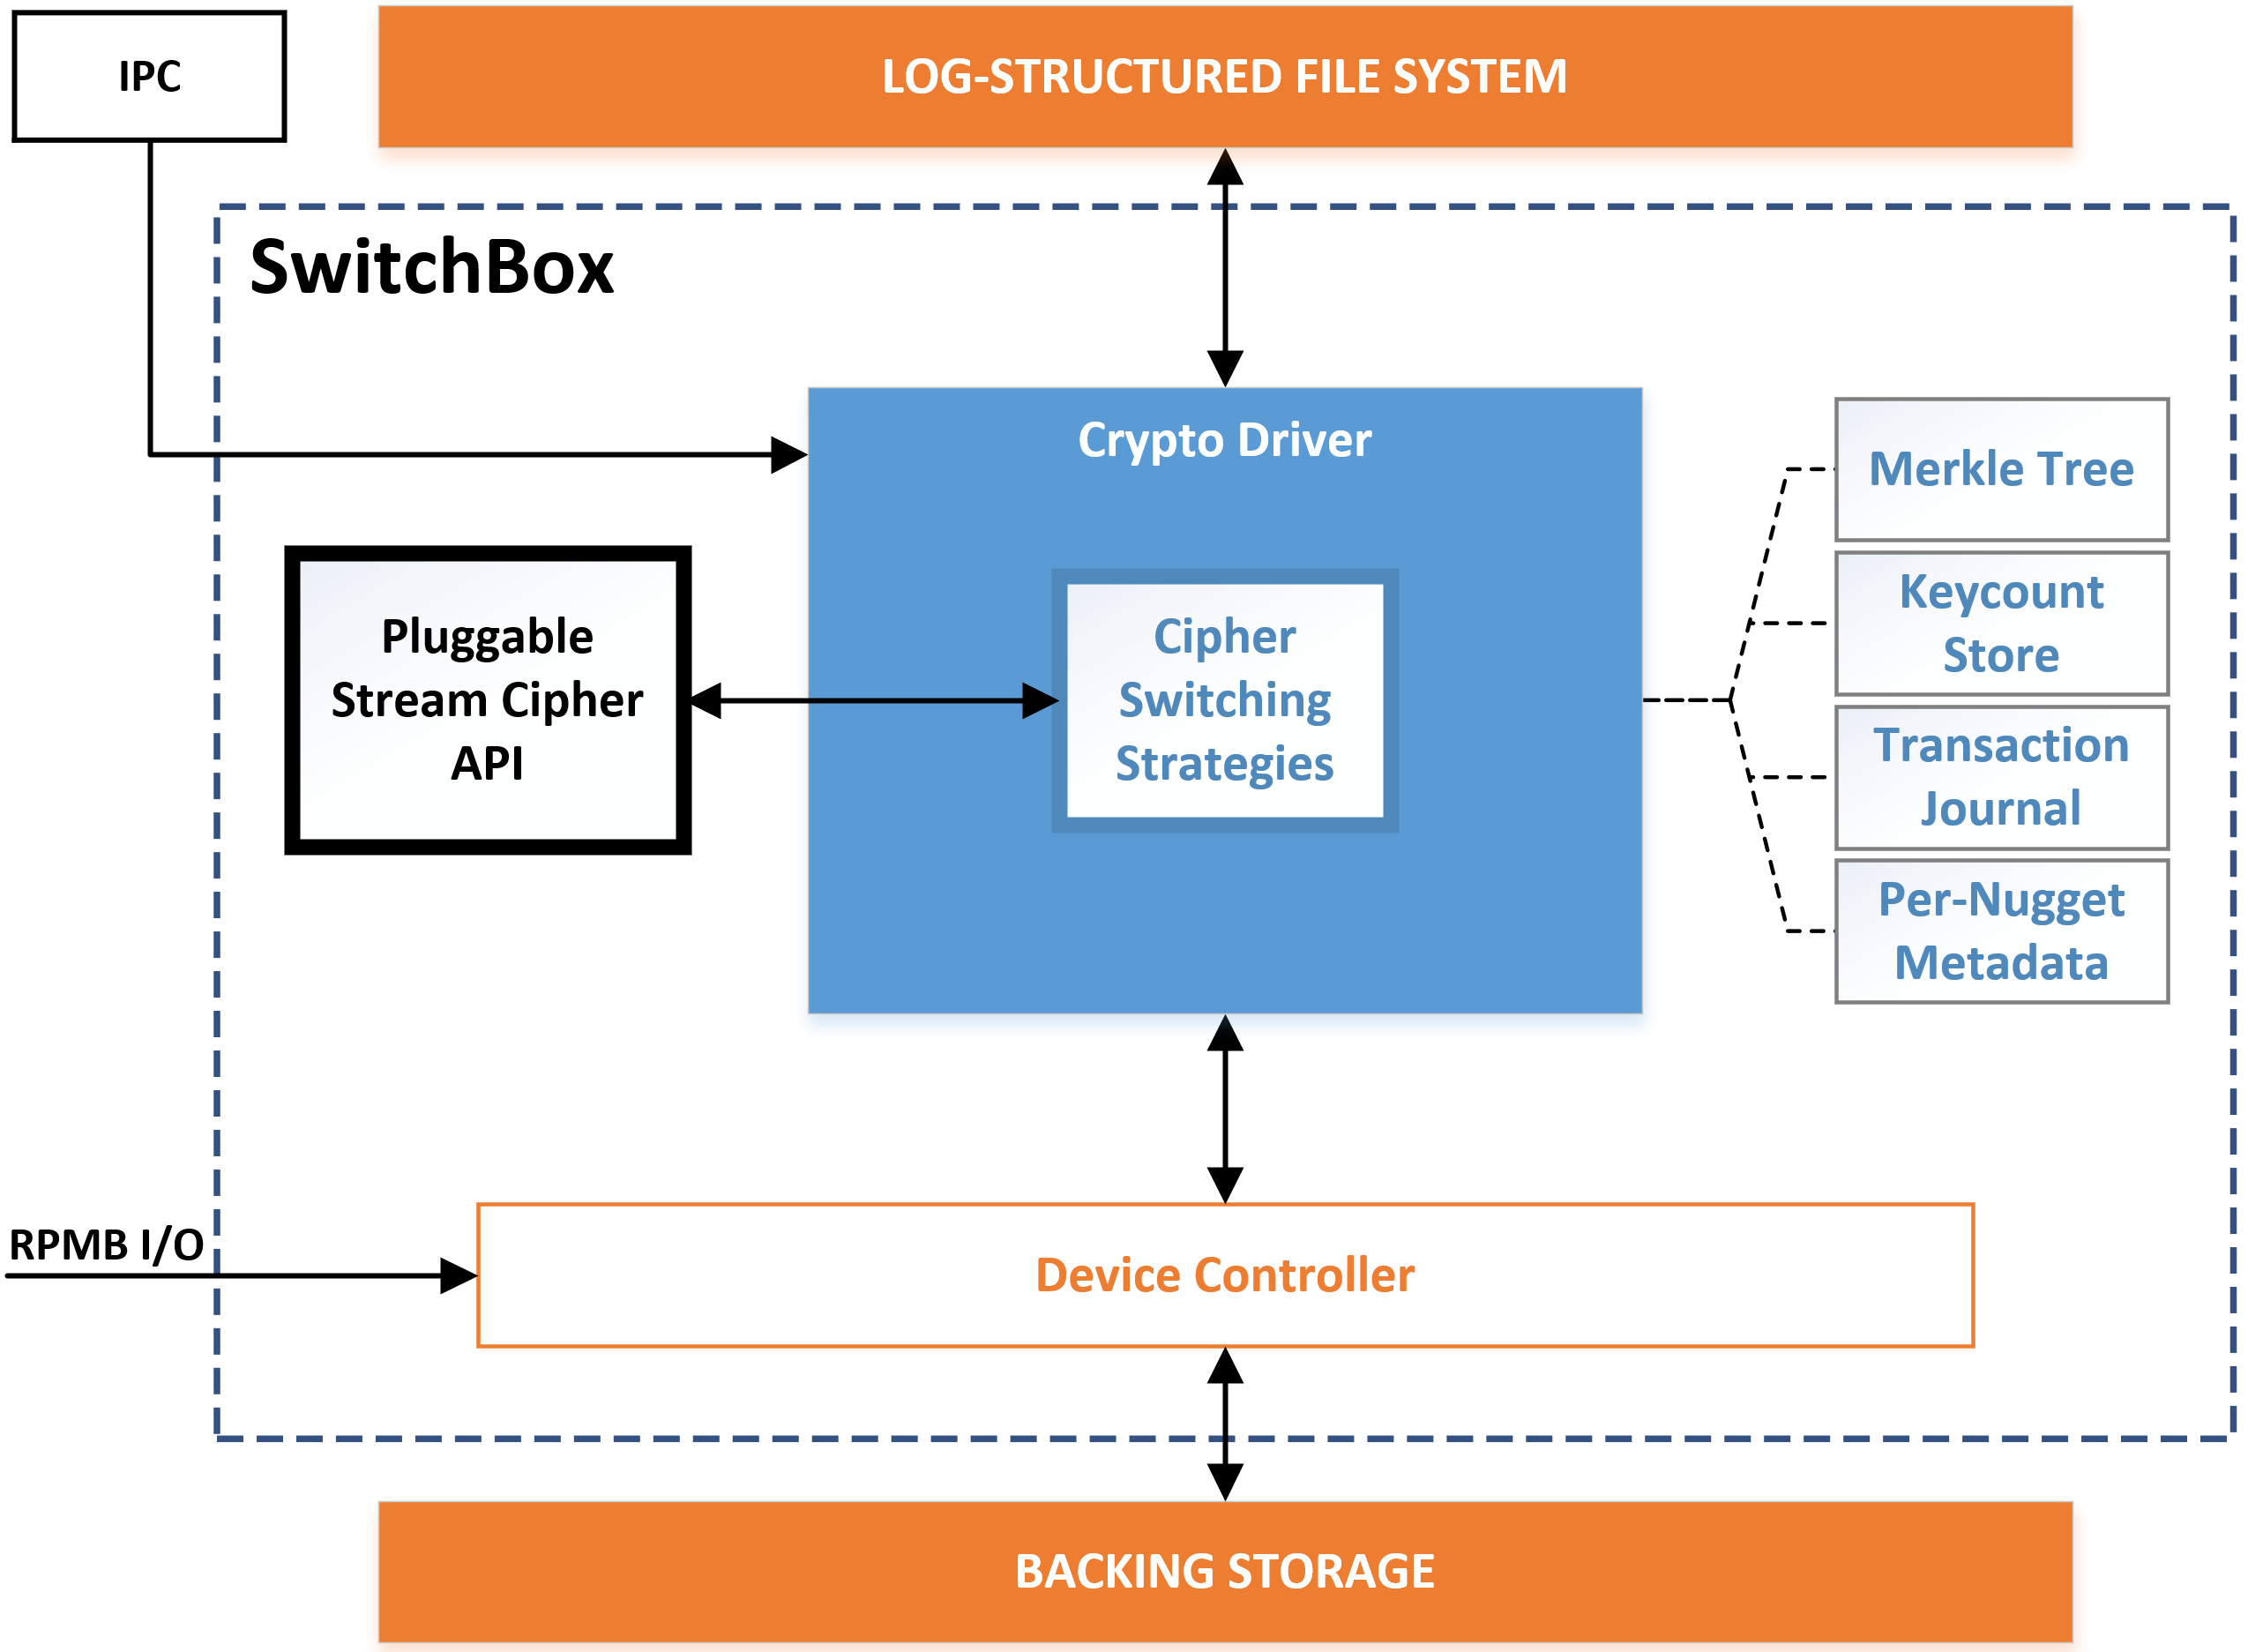
\includegraphics[width=\linewidth]{overview.png}
   \caption{Overview of the \SYSTEM{} construction.}\label{fig:overview}
\end{figure}

\section{\SYSTEM{} Design}\label{sec:design}

\TODO{How much of the original StrongBox should be explained here? Is
this too much? Too little?}

\SYSTEM{}, like StrongBox, is a translation layer positioned between the block
layer and the operating system's virtual file system~\cite{StrongBox}. There are
several places \SYSTEM{} could be implemented in the system stack: as part of an
actual kernel Log-structured File System (LFS) module like the F2FS filesystem,
as a block device or virtual block device in the manner of dm-crypt, or within a
device controller such as an SSD drive controller's FTL~\cite{StrongBox}.

\figref{overview} illustrates the \SYSTEM{} design. \SYSTEM{} manages five
metadata components: an in-memory \emph{Merkle Tree}; two drive-backed byte
arrays, \ie{the \emph{Keycount Store} and the \emph{Transaction Journal}}; a
globally persistent cryptographically secure monotonic counter; and a flexible
drive-backed store for per-nugget cipher-specific metadata. For our
monotonic counter implementation, we used a \emph{Replay Protected Memory Block}
(RPMB).

These five components are tightly integrated into the cryptographic driver,
which handles data encryption, decryption, overwrite detection, integrity
protection, and the application of cipher switching strategies. The
cryptographic driver interacts with 1) the overlying LFS through traditional I/O
passed through the Linux Virtual Filesystem Switch (VFS) as well as 2) the
underlying backing store through the device controller block I/O layer.

\begin{figure}[t]
 \centering
  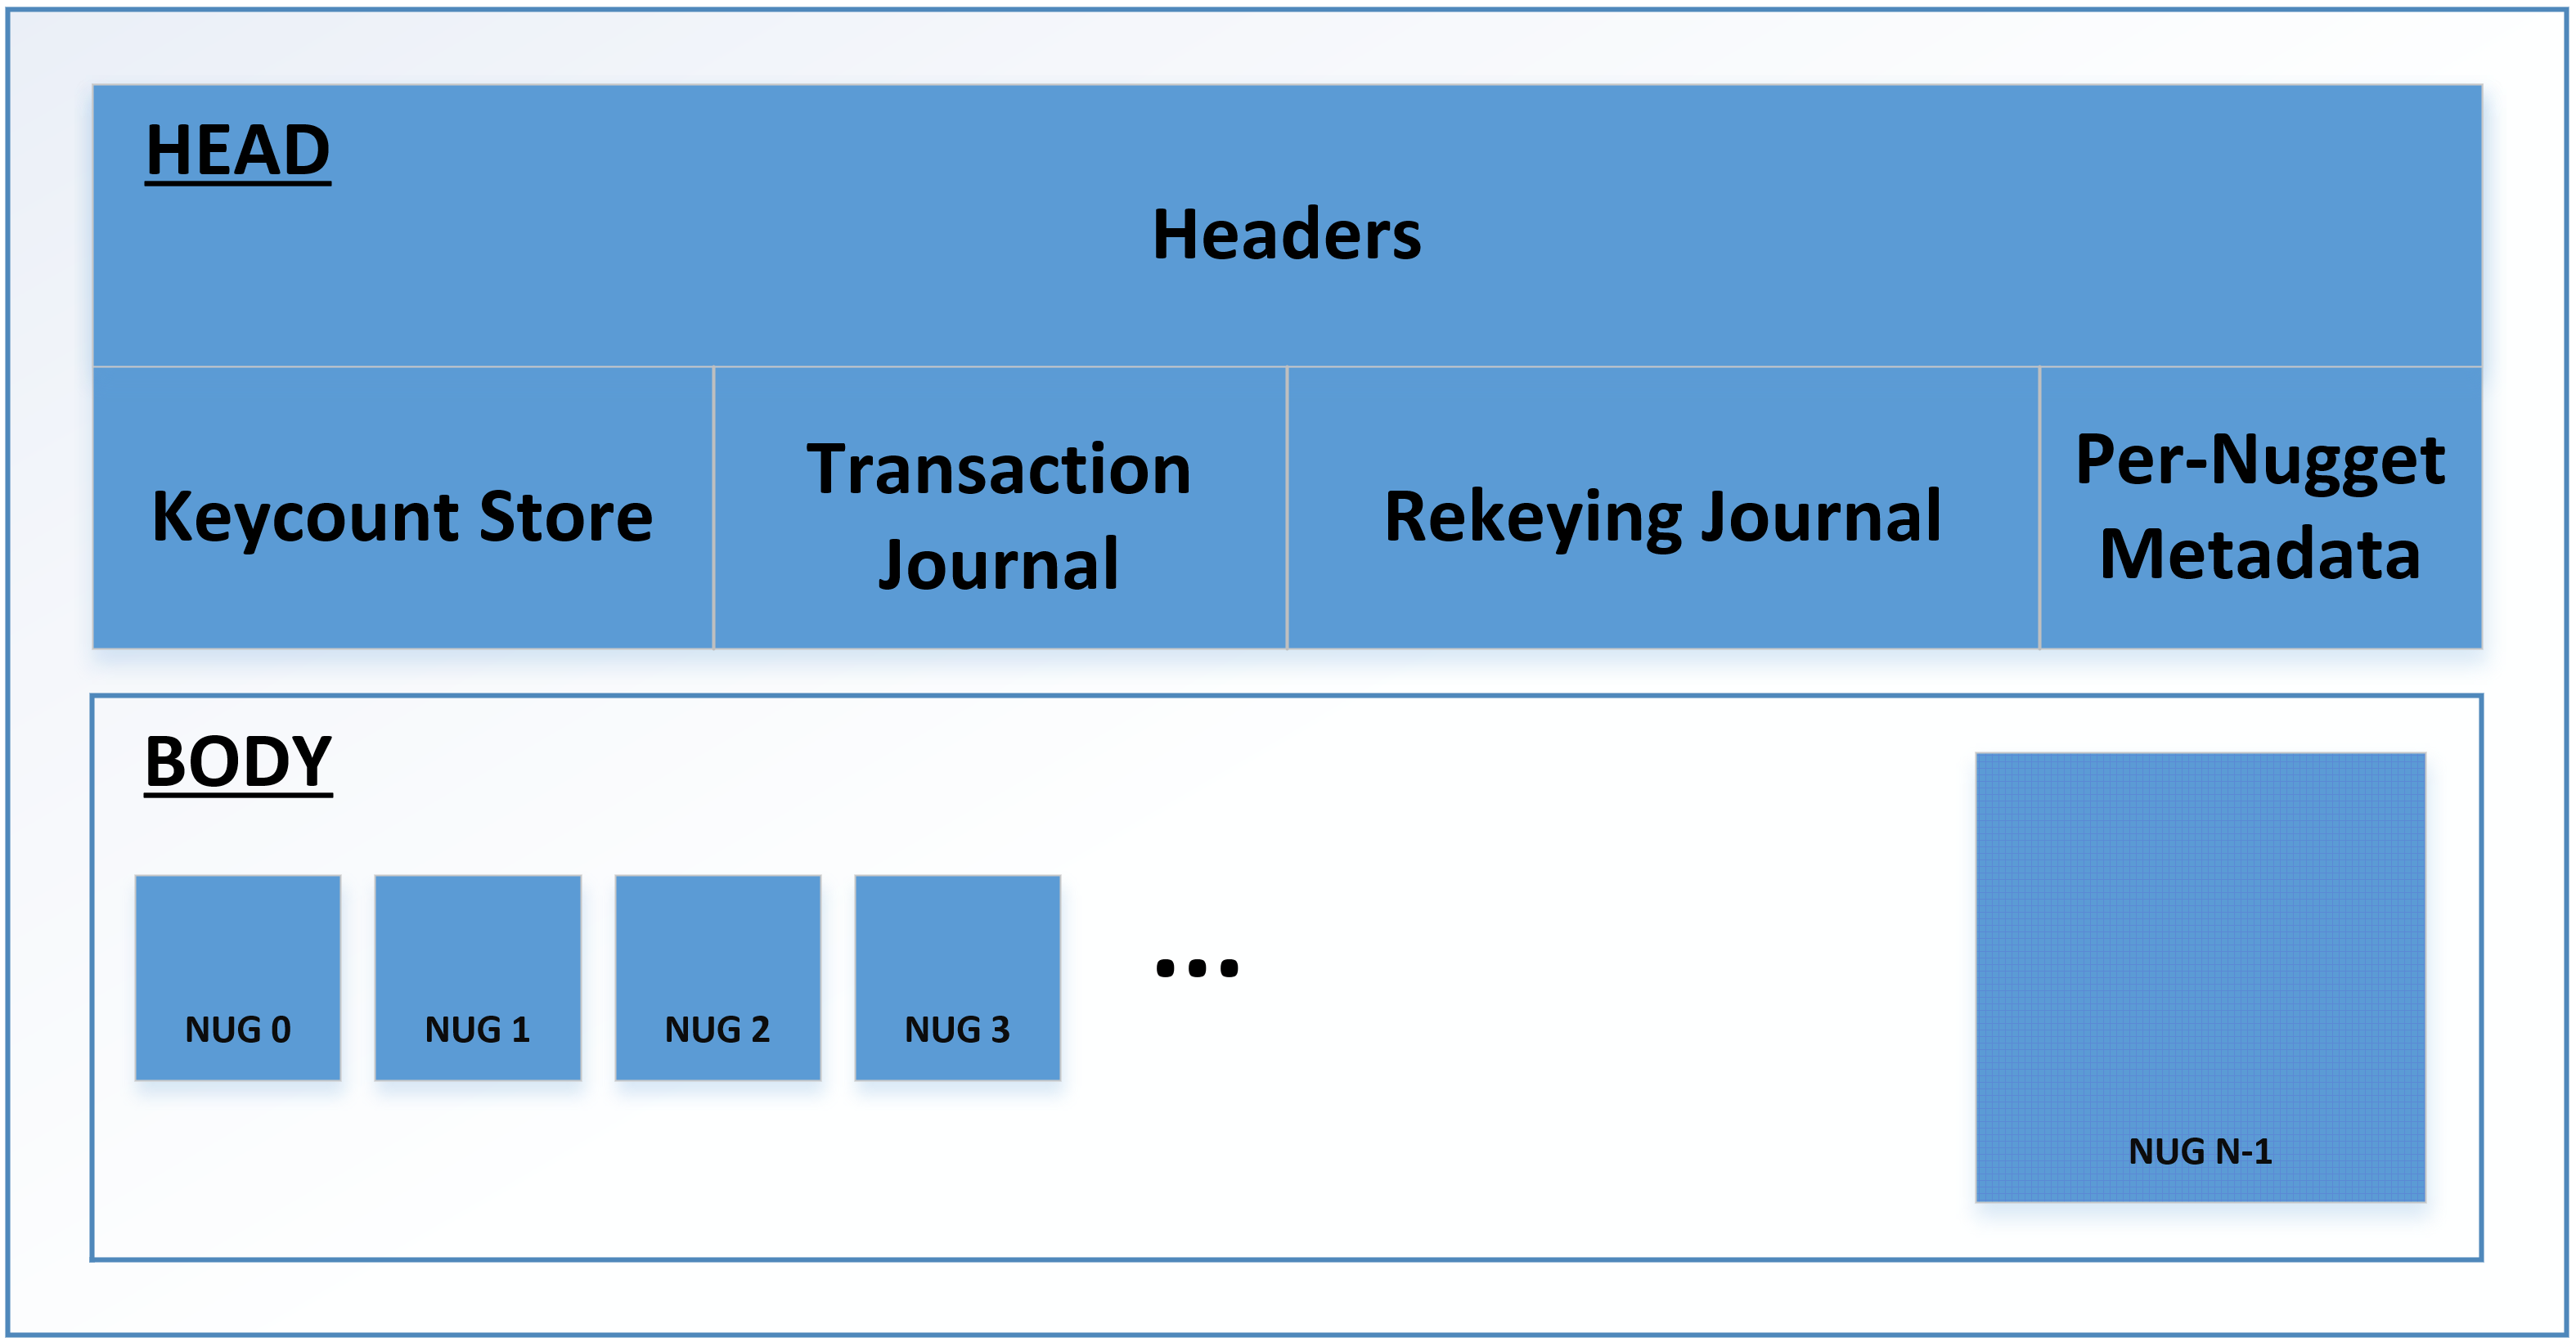
\includegraphics[width=\linewidth]{backstore.png}
   \caption{Layout of \SYSTEM{}'s backing storage.}\label{fig:backstore}
\end{figure}

The backing store is the storage medium \SYSTEM{} operates on. The layout of the
backing store is illustrated with \figref{backstore}. \TODO{Do we redescribe the
backing store from StrongBox, or should we link to the original paper? Or should
we skip talking about the backing store at all and just briefly describe nuggets
here? It's not very different from StrongBox's. An extra header was added.}

In the rest of this section, we describe our cipher switching strategies,
pluggable stream cipher API, and related design challenges with these
components. This is followed by an explanation of implementation-specific
details and a discussion of the overall implications and limitations of
\SYSTEM{}'s design.

\subsection{Cipher Switching Strategies}

Upon initialization, prior work requires a single cipher to be selected. The
specified cipher---ideally along the pareto frontier---is then used to encrypt
and decrypt all data on the filesystem. With \SYSTEM{}, however, \emph{a pair of
ciphers are selected along the pareto frontier} upon initialization depending on
the concerns of the user. These ciphers are the static configuration points
between which \SYSTEM{} navigates.

Switching ciphers dynamically allows \SYSTEM{} to achieve optimal configuration
points that are otherwise unachievable with prior work. However, it is entirely
non-trivial to determine \emph{when} to switch ciphers and \emph{where} to
direct cipher output.

Hence, cipher switching \emph{strategies} are the mechanism by which \SYSTEM{}
can effectively transition nuggets between different encrypted states
dynamically, thus providing a mechanism to navigate the tradeoff space presented
in
\figref{fig:40mb-read-with-forward}. \TODO{Expound on this all more? Reword?}

\subsubsection{Forward}

The forward switching strategy allows each individual nugget to exist encrypted
using one cipher or the other. Other parts of the operating system can indicate
which cipher \SYSTEM{} should be using to interact with the backing store at any
time. When \SYSTEM{} receives the signal it is determined that the system should be interacting with nuggets
encrypted in a specific form.

\subsubsection{Selective}

\TODO{A paragraph}

\subsubsection{Mirrored}

\TODO{A paragraph}

\subsection{Pluggable Stream Cipher API}

\TODO{Some paragraphs}

\subsection{Challenges}

\TODO{Performance overhead paragraph}

\TODO{Spatial overhead paragraph}

\subsection{Implementation}

Our \SYSTEM{} implementation consists of 9,491 lines of C code; our test suite
consists of 6,077 lines of C code. All together, our solution is comprised of
15,568 lines of C code. \SYSTEM{} uses OpenSSL version 1.1.0h and LibSodium
version 1.0.12 for its AES-XTS implementation. \TODO{Sentence or two about the
origin of estream cipher implementations}. As with the original StrongBox, the
Merkle Tree implementation is from the Secure Block Device~\cite{SBD}. \SYSTEM{}
implementation is publicly available open-source.\footnote{\SystemURI}.

For a fair comparison with the original StrongBox implementation, we mirror
their use of the BUSE~\cite{BUSE} virtual block device as our device controller.
BUSE is a thin (200 LoC) wrapper around the standard Linux Network Block Device
(NBD). Buse allows an operating system to transact block I/O requests to and
from virtual block devices exposed via domain socket.

For the purposes of our implementation, we make the choice of ciphers binary:
either the system wants \SYSTEM{} to access the backing store using the primary
cipher or the secondary cipher. However, there is no technical limitation
preventing various different nuggets encrypted with three, four, or more unique
ciphers from co-existing on the backing store.

\subsubsection{Indicating a cipher switch should occur}

When the system should be using one cipher over the other to interact with the
backing store, this intent is communicated via POSIX message queue in our
implementation. It is not a requirement of \SYSTEM{} that a POSIX message queue
be used over any other method of inter-process communication so long as
\SYSTEM{} is notified asynchronously when the wider system desires one cipher be
active over the other.

\subsection{Discussion}




